\باب{ابتدائی معلومات}
اس باب میں ان معلومات کو پیش کیا گیا ہے جنہیں جانتے ہوئے احصاء کو سمجھا جا سکتا ہے۔

\حصہ{حقیقی اعداد اور حقیقی خط}
اس حصہ میں حقیقی اعداد، عدم مساوات، وقفہ اور مطلق قیمتوں پر غور کیا جائے گا۔

\جزوحصہء{حقیقی اعداد اور حقیقی خط}
احصاء کا بیشتر حصہ حقیقی عددی نظام کے خواص پر مبنی ہے۔\اصطلاح{حقیقی اعداد}\فرہنگ{حقیقی!اعداد}\حاشیہب{real numbers}\فرہنگ{numbers!real} وہ اعداد ہیں جنہیں اعشاری صورت میں لکھنا ممکن ہو، مثلاً:
\begin{align*}
-\frac{3}{4}&=-0.75000\cdots\\
\frac{1}{3}&=0.33333\cdots\\
\sqrt{2}&=1.4142\cdots
\end{align*}
ہندسوں کا  ہمیشہ تک چلتے رہنے کو نقطوں \نقطے سے ظاہر کیا گیا ہے۔

حقیقی اعداد کو لکیر پر بطور نقطے ظاہر کیا جا سکتا ہے۔اس لکیر کو \اصطلاح{حقیقی خط}\فرہنگ{حقیقی!خط}\حاشیہب{real line}\فرہنگ{real!line} کہتے ہیں۔
\begin{center}
\begin{tikzpicture}[x=1.5cm,font=\footnotesize]
\centering
\draw(-2.5,0)--(4.2,0);
\foreach \x in {0,1,2,3,4}{\draw(\x,0)node[below]{$\x$}--++(0,0.1);}
\draw(-2,0)node[below,xshift={(-0.15cm)}]{$-1$}--++(0,0.1);
\draw(-1,0)node[below,xshift={(-0.15cm)}]{$-2$}--++(0,0.1);
\draw(-3/4,0)node[below]{$-\tfrac{3}{4}$}--++(0,0.1);
\draw(1/3,0)node[below]{$\tfrac{1}{3}$}--++(0,0.1);
\draw(1.4142,0)node[below]{$\sqrt{2}$}--++(0,0.1);
\draw(3.142,0)node[below]{$\pi$}--++(0,0.1);
\end{tikzpicture}
\end{center}
\عددی{\Re} کی علامت حقیقی عددی نظام یا، اس کے مترادف، حقیقی خط کو ظاہر کرتی ہے۔

\جزوحصہء{حقیقی اعداد کے خواص}  
حقیقی اعداد کے خواص تین گروہوں میں تقسیم کیے جا سکتے ہیں: الجبرائی خواص، خواص درجہ، اور کاملیت۔ الجبرائی خواص کہتی ہیں کہ حساب کے عمومی قواعد کے تحت حقیقی اعداد کو جمع، تفریق، ضرب اور (ماسوائے \عددی{0} سے) تقسیم   کرتے ہوئے مزید حقیقی اعداد پیدا کیے جا سکتے ہیں۔آپ کبھی بھی \عددی{0} سے تقسیم نہیں کر سکتے ہیں۔

حقیقی اعداد کی خواص درج ذیل ہیں۔\\
\begin{mdframed}[frametitlerulewidth=10pt,frametitle={قواعد برائے عدم مساوات}]

اگر \عددی{a}، \عددی{b} اور \عددی{c} حقیقی اعداد ہوں، تب:
\begin{enumerate}[1.]
\item
$a+c<b+c\impliedby a<b$
\item
$a-c<b-c\impliedby a<b$
\item
$ac<bc\impliedby a<b \,\text{اور}\, c>0$
\item
$bc<ac\impliedby a<b\, \text{اور}\, c<0$\quad 
خصوصی صورت:
$-b<-a\impliedby a<b$
\item
$\frac{1}{a}>0\impliedby a>0$
\item
اگر \عددی{a} اور \عددی{b} دونوں مثبت یا دونوں منفی ہوں تب 
$\frac{1}{b}<\frac{1}{a}\impliedby a<b$
\end{enumerate}
\end{mdframed}
درج بالا میں $a+c<b+c\impliedby a<b$ کہتا ہے کہ اگر \عددی{a} کی قیمت \عددی{b} کی قیمت سے کم ہو تب اس سے آپ اخذ کر سکتے ہیں کہ \عددی{a+c} کی قیمت \عددی{b+c} کی قیمت سے کم ہو گی۔دھیان رہے کہ عدم مساوات کو مثبت عدد سے ضرب دینے سے عدم مساوات اپنی صورت برقرار رکھتی ہے جبکہ اس کو منفی عدد سے ضرب دینے سے عدم مساوات کی علامت الٹ ہو جاتی ہے۔ 

حقیقی عددی نظام کی کاملیت زیادہ گہری خاصیت ہے جس کی درست تعریف مشکل ہے۔ہم کہہ سکتے ہیں کہ حقیقی اعداد کی تعداد اتنی ہے کہ یہ حقیقی خط کو مکمل کر پاتے ہیں، یعنی، حقیقی خط پر کوئی "سراخ" یا "درز" نہیں پایا جاتا ہے۔ احصاء کے کئی مسئلوں کا دارومدار حقیقی عددی نظام کے مکمل ہونے پر ہے۔کاملیت کا موضوع زیادہ اعلیٰ درجہ حساب کا حصہ ہے اور اس پر مزید بحث نہیں کی جائے گی۔  

\جزوحصہء{\عددی{\Re} کا ذیلی سلسلہ}
ہم حقیقی اعداد کے تین خصوصی ذیلی \اصطلاح{سلسلوں}\فرہنگ{سلسلہ}\حاشیہب{sets}\فرہنگ{sets} کی وضاحت کرنا چاہتے ہیں۔
\begin{enumerate}[1.]
\item
\اصطلاح{قدرتی اعداد}\فرہنگ{اعداد!حقیقی}\حاشیہب{natural numbers}\فرہنگ{numbers!natural}، یعنی \عددی{1}،\عددی{2}،\عددی{3}،\عددی{4}،\نقطے
\item
\اصطلاح{عدد صحیح}، یعنی \عددی{0}، \عددی{\mp1}، \عددی{\mp2}، \عددی{\mp3}،\نقطے
\item
\اصطلاح{ناطق اعداد}\فرہنگ{اعداد!ناطق}\حاشیہب{rational numbers}\فرہنگ{numbers!rational}، یعنی وہ اعداد جنہیں کسر \عددی{\tfrac{m}{n}} کی صورت میں لکھنا ممکن ہو جہاں \عددی{m} اور \عددی{n} عددی صحیح ہیں اور \عددی{n} غیر صفر \عددی{n\ne 0} ہے۔اس کی مثال درج ذیل ہیں۔
\begin{align*}
\frac{1}{3},\quad -\frac{4}{9},\quad \frac{200}{13}, \quad 57=\frac{57}{1}
\end{align*} 
\end{enumerate}
ناطق اعداد کو اعشاری روپ میں لکھتے ہوئے حقیقی اعداد کی دو صورتیں ممکن ہیں۔\\
(الف) \quad
مختتم (جو لامتناہی صفروں پر اختتام ہوتی ہے)، مثلاً
\begin{align*}
\frac{3}{4}=0.75000\cdots=0.75
\end{align*}
(ب)\quad
دہراتا (جو ایسے ہندسوں پر اختتام ہوتا ہے جو بار بار دہراتے رہتے ہیں)، مثلاً
\begin{align*}
\frac{23}{11}=2.090909\cdots=2.\overline{09}
\end{align*}

ناطق اعداد  کا سلسلہ حقیقی اعداد کی  الجبرائی خواص اور خواص درجہ رکھتے ہیں البتہ یہ کاملیت کی خاصیت نہیں رکھتے ہیں، مثلاً، ایسا کوئی ناطق عدد نہیں پایا جاتا ہے جس کا مربع \عددی{2} ہو۔یوں ناطق خط میں اس نقطے پر "سراخ" پایا جاتا ہے جہاں \عددی{\sqrt{2}} کو ہونا چاہیے تھا۔

وہ حقیقی اعداد جو ناطق نہ ہوں \اصطلاح{غیر ناطق اعداد}\فرہنگ{اعداد!غیر ناطق}\حاشیہب{irrational numbers}\فرہنگ{numbers!irrational} کہلاتے ہیں۔غیر ناطق اعداد کو اعشاری روپ میں لکھنے سے نا مختتم اور نا ہی دہراتی صورت ملتی ہے۔ناطق اعداد  کی مثالیں \عددی{\pi}، \عددی{\sqrt{2}} اور \عددی{\log_{10}{3}} ہیں۔

\جزوحصہء{وقفہ}
حقیقی خط کا ایسا ذیلی سلسلہ جس میں کم سے کم دو اعداد پائے جاتے ہوں اور جس میں ہر دو ارکان کے بیچ تمام  حقیقی اعداد بھی  شامل ہوں \اصطلاح{وقفہ}\فرہنگ{وقفہ}\حاشیہب{interval}\فرہنگ{interval} کہلاتا ہے۔ مثال کے طور تمام حقیقی اعداد \عددی{x} کا سلسلہ جہاں \عددی{x>4} ہو وقفہ ہے۔اسی طرح تمام \عددی{x} کا سلسلہ جہاں \عددی{-4\le x\le 8} ہو بھی وقفہ ہے۔ اس کے برعکس تمام غیر صفر حقیقی اعداد وقفہ نہیں ہیں چونکہ \عددی{0} اس کا حصہ نہیں ہے لہٰذا \عددی{-1} اور \عددی{1} کے بیچ تمام اعداد سلسلہ کا حصہ نہیں ہیں۔

جیومیٹریائی طور پر حقیقی خط پر قطع یا شعاع یا پورے حقیقی خط کو سلسلہ ظاہر کرتا ہے۔خطی قطع \اصطلاح{متناہی وقفہ}\فرہنگ{وقفہ!متناہی}\حاشیہب{finite interval}\فرہنگ{interval!finite} جبکہ شعاع یا پورا حقیقی خط \اصطلاح{لامتناہی وقفہ}\فرہنگ{وقفہ!لا متناہی}\حاشیہب{infinite interval}\فرہنگ{interval!infinite} کہلاتے ہیں۔

اگر متناہی وقفہ کے دونوں سر بھی وقفہ کا حصہ ہوں تب یہ \اصطلاح{بند}\فرہنگ{بند}\حاشیہب{closed}\فرہنگ{closed} کہلائے گا، اگر اس کا ایک سر وقفہ کا حصہ ہو تب یہ \اصطلاح{نصف کھلا}\فرہنگ{نصف کھلا}\حاشیہب{half-open}\فرہنگ{half-open} کہلاتا ہے اور اگر دونوں سر وقفہ کا حصہ  نہ ہوں تب یہ \اصطلاح{کھلا}\فرہنگ{کھلا}\حاشیہب{open}\فرہنگ{open} کہلاتا ہے۔وقفے کے سروں کو \اصطلاح{سرحدی نقطے}\فرہنگ{سرحدی!نقطے}\حاشیہب{boundary points}\فرہنگ{boundary!points} بھی کہتے ہیں۔یہ وقفہ کی \اصطلاح{سرحد}\فرہنگ{سرحد}\حاشیہب{boundary}\فرہنگ{boundary}  ہیں۔ وقفہ کے باقی نقطوں کو \اصطلاح{اندرونی نقطے}\فرہنگ{اندرونی نقطے}\حاشیہب{interior points}\فرہنگ{interior!points} کہتے ہیں۔تمام اندرونی نقطوں کو وقفہ کی \اصطلاح{اندرون}\فرہنگ{اندرون}\حاشیہب{interior}\فرہنگ{interior} کہتے ہیں۔
\begin{mdframed}[frametitle={وقفوں کی قسمیں}]
\begin{tabular}{cccc}
&علامت& سلسلہ&ترسیم\\
متناہی&$(a,b)$ &$\{x|a<x<b\}$&\begin{tikzpicture}[baseline] \centering  \draw[-latex](-0.5,0)--(3.5,0);\draw[thick](0,0)--(3,0); \draw(0,0)node[ocirc]{}node[below]{$a$} (3,0)node[ocirc]{}node[below]{$b$}; \end{tikzpicture}\\
&$[a,b]$&$\{x|a\le x\le b\}$&\begin{tikzpicture}[baseline] \centering  \draw[-latex](-0.5,0)--(3.5,0);\draw[thick](0,0)--(3,0);  \draw(0,0)node[circ]{}node[below]{$a$} (3,0)node[circ]{}node[below]{$b$}; \end{tikzpicture}\\
&$[a,b)$&$\{x|a\le x <b\}$&\begin{tikzpicture}[baseline] \centering  \draw[-latex](-0.5,0)--(3.5,0);\draw[thick](0,0)--(3,0);  \draw(0,0)node[circ]{}node[below]{$a$} (3,0)node[ocirc]{}node[below]{$b$}; \end{tikzpicture}\\
&$(a,b]$&$\{x|a<x\le b\}$&\begin{tikzpicture}[baseline] \centering  \draw[-latex](-0.5,0)--(3.5,0);\draw[thick](0,0)--(3,0);  \draw(0,0)node[ocirc]{}node[below]{$a$} (3,0)node[circ]{}node[below]{$b$}; \end{tikzpicture}\\
لا متناہی&$(a,\infty)$&$\{x|x>a\}$&\begin{tikzpicture}[baseline] \centering  \draw[-latex](-0.5,0)--(3.5,0);\draw[thick,-latex](0,0)--(3.5,0);  \draw(0,0)node[ocirc]{}node[below]{$a$}; \end{tikzpicture}\\
&$[a,\infty)$&$\{x|x\ge a\}$&\begin{tikzpicture}[baseline] \centering  \draw[-latex](-0.5,0)--(3.5,0);\draw[thick,-latex](0,0)--(3.5,0);  \draw(0,0)node[circ]{}node[below]{$a$}; \end{tikzpicture}\\
&$(-\infty,b)$&$\{x|x<b\}$&\begin{tikzpicture}[baseline] \centering  \draw[-latex](-0.5,0)--(3.5,0);\draw[thick](-0.5,0)--(3,0);  \draw(3,0)node[ocirc]{}node[below]{$b$}; \end{tikzpicture}\\
&$(-\infty,b]$&$\{x|x\le b\}$&\begin{tikzpicture}[baseline] \centering  \draw[-latex](-0.5,0)--(3.5,0);\draw[thick](-0.5,0)--(3,0);  \draw(3,0)node[circ]{}node[below]{$b$}; \end{tikzpicture}\\
&$(-\infty,\infty)$&$\Re$&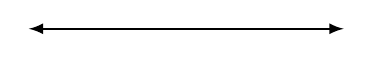
\begin{tikzpicture} \centering  \draw[latex-latex,thick](-0.5,0)--(3.5,0); \end{tikzpicture}\\
\end{tabular}
\end{mdframed}


\جزوحصہء{عدم مساوات کا حل}
\عددی{x} پر مبنی عدم مساوات کو حل کرتے ہوئے اعداد کا وقفہ یا وقفے تلاش کرنے کو عدم مساوات کا حل کہتے ہیں۔

%=====================
\ابتدا{مثال}\شناخت{مثال_ابتدا_عدم_مساوات_الف}
\begin{multicols}{3}
\begin{enumerate}[1)]
\item
 $2x-4<x+1$
\item
$-\tfrac{x}{3}<x-1$
\item
$\tfrac{2}{x-1}\ge 4$
\end{enumerate}
\end{multicols}
حل:
\begin{enumerate}[1)]
\item
\begin{align*}
2x-4&<x+1&&\\
2x&<x+5&&\text{\RL{دونوں ہاتھ $4$ جمع کریں}}\\
x&<5&& \text{دونوں ہاتھ سے $x$ منفی کریں}
\end{align*}
%
\begin{center}
\begin{tikzpicture}
\centering
\draw[-latex](-0.5,0)--(3.5,0)node[right]{$x$};
\draw[thick] (-0.5,0)--(3,0);
\draw(3,0)node[ocirc]{}node[below]{$5$}--++(0,0.1);
\end{tikzpicture}
\end{center}
حل سلسلہ وقفہ \عددی{(-\infty,5)} ہے۔\\
\item
\begin{align*}
-\frac{x}{3}&<x-1\\
-x&<3x-3&&\text{\RL{دونوں ہاتھ کو $3$ سے ضرب دیں}}\\
0&<4x-3&&\text{دونوں ہاتھ کے ساتھ $x$ جمع کریں}\\
3&<4x&&\text{\RL{دونوں ہاتھ کے ساتھ $3$ جمع کریں}}\\
\frac{3}{4}&<x&&\text{\RL{دونوں ہاتھ کو $3$ سے تقسیم کریں}}
\end{align*}
%
\begin{center}
\begin{tikzpicture}
\centering
\draw[-latex](-0.5,0)--(3.5,0)node[right]{$x$};
\draw[thick,-latex] (2,0)--(3.5,0);
\draw(2,0)node[ocirc]{}node[below]{$\tfrac{3}{4}$}--++(0,0.1);
\end{tikzpicture}
\end{center}
وقفہ \عددی{(\tfrac{3}{4},\infty)} حل سلسلہ ہے۔\\
\item
عدم مساوات \عددی{\tfrac{2}{x-1}\ge 4} صرف \عددی{x>1} کی صورت میں درست ہو گا چونکہ \عددی{x<1} کی صورت میں بایاں ہاتھ منفی ہو گا اور \عددی{x=1} پر بایاں ہاتھ غیر متعین ہے۔عدم مساوات کے دونوں ہاتھ کو \عددی{x-1} سے ضرب دیتے ہوئے عدم مساوات برقرار رہتا ہے۔
\begin{align*}
\frac{2}{x-1}&\ge 4\\
2&\ge 4x-4&&\text{\RL{دونوں ہاتھ کو $x-1$ سے ضرب دیں}}\\
6&\ge 4x&&\text{\RL{دونوں ہاتھ کے ساتھ $4$ جمع کریں}}\\
\frac{3}{2}&\ge x&&\text{\RL{دونوں ہاتھ کو $4$ سے تقسیم کریں}}
\end{align*}
%
\begin{center}
\begin{tikzpicture}
\draw[-latex](-0.5,0)--(3.5,0)node[right]{$x$};
\draw[thick] (2,0)--(2.5,0);
\draw(2.5,0)node[circ]{}node[below]{$\tfrac{3}{2}$}--++(0,0.1);
\draw(2,0)node[ocirc]{}node[below]{$1$}--++(0,0.1);
\end{tikzpicture}
\end{center}
حل سلسلہ نصف کھلا وقفہ \عددی{(1,\tfrac{3}{2}]} ہے۔
\end{enumerate}
\انتہا{مثال}
%=========================
\جزوحصہء{مطلق قیمت}
عدد \عددی{x} کی \اصطلاح{مطلق قیمت}\فرہنگ{مطلق قیمت}\حاشیہب{absolute value}\فرہنگ{absolute value} جس کو \عددی{\abs{x}} سے ظاہر کیا جاتا ہے کہ تعریف درج ذیل ہے۔
\begin{align*}
\abs{x}=
\begin{cases}
\phantom{-}x&x\ge 0\\
-x&x<0
\end{cases}
\end{align*}

%======================
\ابتدا{مثال}
$\abs{0.88}=0.88,\quad \abs{0}=0,\quad \abs{-13}=-(-13)=13,\quad \abs{-\abs{a}}=\abs{a}$
\انتہا{مثال}
%=========================

دھیان رہے کہ ہر حقیقی عدد کی مطلق قیمت غیر منفی \عددی{\abs{x}\ge } ہو گی اور صرف \عددی{x=0} کی صورت میں \عددی{\abs{x}=0} ہو گا۔چونکہ \عددی{a} کی غیر منفی  جذر کو \عددی{\sqrt{a}} سے ظاہر کیا جاتا ہے لہٰذا \عددی{\abs{x}} کی متبادل تعریف درج ذیل لی جا سکتی ہے۔
\begin{align*}
\abs{x}=\sqrt{x^2}
\end{align*} 
آپ \عددی{\sqrt{a^2}=\abs{a}} لکھ سکتے ہیں جبکہ \عددی{\sqrt{a^2}=a} صرف مثبت \عددی{a} کی صورت میں درست ہو گا۔ 

جیومیٹریائی طور پر حقیقی خط پر مبدا \عددی{0} سے \عددی{x} تک فاصلے کو \عددی{\abs{x}} ظاہر کرتی ہے۔زیادہ عمومی طور پر (شکل \حوالہ{شکل_ابتدائی_مطلق_جیومیٹریائی_مطلب}) 
\begin{align*}
\abs{x-y}=\text{\RL{$\,x\,$ اور $\,y\,$ کے بیچ فاصلہ}}
\end{align*}
ہو گا۔
\begin{figure}
\centering
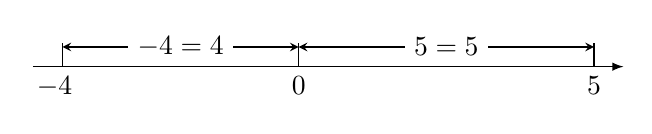
\begin{tikzpicture}[x=0.75cm]
\draw[stealth-stealth] (-4,0.25)--(0,0.25)node[pos=0.5,fill=white]{$\abs{-4}=4$};
\draw[stealth-stealth] (0,0.25)--(5,0.25)node[pos=0.5,fill=white]{$\abs{5}=5$};
\draw[-latex](-4.5,0)--(5.5,0);
\draw(-4,0)node[below,xshift={-1mm}]{$-4$}--++(0,0.3);
\draw(0,0)node[below]{$0$}--++(0,0.3);
\draw(5,0)node[below]{$5$}--++(0,0.3);
\end{tikzpicture}
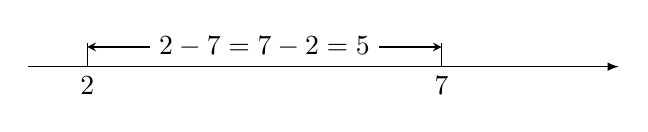
\begin{tikzpicture}[x=0.75cm]
\draw[stealth-stealth](1,0.25)--(7,0.25)node[pos=0.5,fill=white]{$\abs{2-7}=\abs{7-2}=5$};
\draw[-latex](0,0)--(10,0);
\draw(1,0)node[below]{$2$}--++(0,0.3);
\draw(7,0)node[below]{$7$}--++(0,0.3);
\end{tikzpicture}
\caption{مطلق قیمت حقیقی خط پر دو نقطوں کے بیچ فاصلہ دیتا ہے۔}
\label{شکل_ابتدائی_مطلق_جیومیٹریائی_مطلب}
\end{figure}
مطلق قیمت کے درج ذیل خواص پائے جاتے ہیں۔
\begin{mdframed}[frametitle={مطلق قیمت کے خواص}]
\begin{enumerate}[1.]
\item{$\abs{-a}=\abs{a}$}\quad
کسی بھی عدد اور نفی عدد  کی مطلق قیمتیں ایک جیسی ہوں گی۔
\item{$\abs{ab}=\abs{a}\abs{b}$}\quad
حاصل ضرب کی مطلق قیمت، مطلق قیمتوں کا حاصل ضرب ہو گا۔
\item{$\abs{\frac{a}{b}}=\frac{\abs{a}}{\abs{b}}$}\quad
حاصل تقسیم کی مطلق قیمت، مطلق قیمتوں کا حاصل تقسیم ہو گا۔
\item{$\abs{a+b}\le \abs{a}+\abs{b}$}\quad
دو اعداد کے مجموعہ کی مطلق قیمت دونوں کے مطلق قیمتوں کے مجموعہ سے کم یا اس کے برابر ہو گی۔اس کو \اصطلاح{تکونی عدم مساوات}\فرہنگ{تکونی عدم مساوات} کہتے ہیں۔
\end{enumerate}
\end{mdframed}

اگر \عددی{a} اور \عددی{b} کی علامتیں مختلف ہوں تب \عددی{\abs{a+b}} کی قیمت \عددی{\abs{a}+\abs{b}} کی قیمت سے کم ہو گی۔اس کے علاوہ ہر صورت \عددی{\abs{a+b}=\abs{a}+\abs{b}} ہو گا۔

\ابتدا{مثال}
\begin{align*}
\abs{-2+6}&=\abs{4}=4<\abs{-2}+\abs{6}=8\\
\abs{2+6}&=\abs{8}=\abs{2}+\abs{6}\\
\abs{-2-6}&=\abs{-8}=8=\abs{-2}+\abs{-6}
\end{align*}
\انتہا{مثال}
%============================
مطلق کی علامت قوسین کی طرح کردار ادا کرتی ہے۔مطلق کی علامت کے اندر جمع، منفی وغیرہ مکمل کرنے کے بعد مطلق قیمت حاصل کی جاتی ہے۔

\ابتدا{مثال} 
مساوات \عددی{\abs{2x-1}=11} کو حل کریں۔\\
حل:\quad
اس مساوات کے تحت \عددی{2x-1=\mp 11} ہو سکتا ہے لہٰذا اس کے دو ممکن جوابات ہیں جو مطلق کی علامت کے بغیر دو مساوات سے حاصل کی جاتی ہیں۔
\begin{gather*}
\begin{aligned}
2x-1&=11\\
2x&=12\\
x&=6
\end{aligned}\quad\quad
\begin{aligned}
2x-1&=-11\\
2x&=-10\\
x&=-5
\end{aligned}
\end{gather*}
یوں \عددی{\abs{2x-1}=11} کا درکار حل \عددی{x=6} اور \عددی{x=-5}  ہے۔
\انتہا{مثال}
%====================

\جزوحصہء{مطلق قیمت والے عدم مساوات}
عدم مساوات \عددی{\abs{a}<D} کہتی ہے کہ مبدا \عددی{0} سے \عددی{a} تک فاصلہ \عددی{D} سے کم ہے۔یوں \عددی{D} اور \عددی{-D} کے بیچ \عددی{a} پایا جائے گا۔

\begin{mdframed}[frametitle={مطلق قیمتیں اور وقفے}]
اگر \عددی{D} کوئی مثبت عدد ہو، تب
\begin{align}
\abs{a}&<D \iff -D<a<D\label{مساوات_ابتدائی_عدم_مساوات_الف}\\
\abs{a}&\le D \iff -D\le a\le D\label{مساوات_ابتدائی_عدم_مساوات_ب}
\end{align}
\end{mdframed}

\ابتدا{مثال}
عدم مساوات \عددی{\abs{x-3}<7} کو حل کریں  اور  حل سلسلہ کو حقیقی خط پر ترسیم کریں۔\\
حل:\quad
\begin{align*}
\abs{x-3}&<7\\
-7<x-3&<7 && \text{\RL{مساوات \حوالہ{مساوات_ابتدائی_عدم_مساوات_الف}}}\\
-7+3<x&<7+3&&\text{\RL{دونوں حصوں کے ساتھ $3$ جمع کریں}}\\
-4<x<&10
\end{align*}
حل سلسلہ کھلا وقفہ \عددی{(-4,10)} ہے۔
\begin{center}
\begin{tikzpicture}
\draw[stealth-stealth](0,0.25)--(2,0.25)node[pos=0.5,fill=white]{$7$};
\draw[stealth-stealth](2,0.25)--(4,0.25)node[pos=0.5,fill=white]{$7$};
\draw[-latex](-0.5,0)--(5,0)node[right]{$x$};
\draw[thick](0,0)node[ocirc]{}node[below]{$-4$}--(4,0)node[ocirc]{}node[below]{$10$};
\draw(2,0)node[below]{$3$}--++(0,0.1);
\end{tikzpicture}
\end{center}
\انتہا{مثال}
%===================
\ابتدا{مثال}
عدم مساوات \عددی{\abs{3-\tfrac{2}{x}}<1} کو حل کریں۔\\
حل:\quad
\begin{align*}
\abs{3-\frac{2}{x}}<1 \iff -1&<3-\frac{2}{x}<1 &&\text{\RL{مساوات \حوالہ{مساوات_ابتدائی_عدم_مساوات_الف}}}\\
-4&<-\frac{2}{x}<-2 && \text{\RL{$3$ منفی کریں}}\\
2&>\frac{1}{x}>1 && \text{\RL{$-\tfrac{1}{2}$ سے ضرب دیں}}\\
\frac{1}{2}&<x<1&&\text{\RL{معکوس لیں}}
\end{align*}

اس مثال میں عدم مساوات پر مختلف حسابی اعمال کا اطلاق کیا گیا۔آپ نے دیکھا کہ منفی عدد سے ضرب دینے سے عدم مساوات الٹ ہو جاتی ہے۔اسی طرح اگر دونوں ہاتھ مثبت ہوں تب  معکوس لینے سے عدم مساوات الٹ ہوتی ہے۔ اصل عدم مساوات اس صورت مطمئن ہو گی جب \عددی{\tfrac{1}{2}<x<1} ہو۔حل سلسلہ کھلا وقفہ \عددی{(\tfrac{1}{2},1)} ہے۔
\انتہا{مثال}
%======================
\ابتدا{مثال}
درج ذیل عدم مساوات حل کریں۔حل سلسلہ ترسیم  کریں۔
\begin{align*}
(\text{الف})\quad \abs{2x-5}&\le1&& (\text{ب})\quad \abs{2x-5}\ge 1
\end{align*} 
حل:\quad (الف)
\begin{align*}
\abs{2x-5}&\le 1\\
-1\le 2x-5&\le1&&\text{\RL{مساوات \حوالہ{مساوات_ابتدائی_عدم_مساوات_ب}}}\\
4\le 2x&\le 6&&\text{\RL{جمع $5$}}\\
2\le x&\le 3&&\text{\RL{تقسیم $2$}}
\end{align*}
حل سلسلہ بند وقفہ \عددی{[2,3]} ہے۔
\begin{center}
\begin{tikzpicture}
\draw[-latex] (-0.5,0)--(4.5,0)node[right]{$x$};
\draw[thick] (1,0)node[circ]{}node[below]{$2$}--(3,0)node[circ]{}node[below]{$3$};
\end{tikzpicture}
\end{center}
(ب)\quad 
\begin{align*}
\begin{array}{c|c}
\multicolumn{2}{c}{\abs{2x-5}\ge 1}\\
\\
2x-5\ge 1&-(2x-5)\ge 1\\
2x\ge 6&2x-5\le -1\\
x\ge 3&2x\le 4\\
&x\le 2
\end{array}
\end{align*}
حل سلسلہ 
$(-\infty,2] \cup [3,\infty)$
 ہے۔
\begin{center}
\begin{tikzpicture}
\draw[-latex] (-0.5,0)--(4.5,0)node[right]{$x$};
\draw[thick] (1,0)node[circ]{}node[below]{$2$}--(-0.5,0);
\draw[thick](3,0)node[circ]{}node[below]{$3$}--(4.5,0);
\end{tikzpicture}
\end{center}
\انتہا{مثال}
%=======================
درج بالا مثال کے دوسرے حل سلسلہ میں وقفوں کی \اصطلاح{اشتراک}\فرہنگ{اشتراک}\حاشیہب{union}\فرہنگ{union} کی علامت \عددی{\cup} استعمال کی گئی ہے۔دو سلسلوں کی اشتراک میں ایک عدد اس صورت پایا جاتا ہے جب یہ عدد کسی ایک یا دونوں سلسلوں میں پایا جاتا ہو۔اسی طرح ہم \اصطلاح{تقاطع}\فرہنگ{تقاطع}\حاشیہب{intersection}\فرہنگ{intersection} کی علامت \عددی{\cap} بھی استعمال کرتے ہیں۔دو سلسلوں کی تقاطع میں ایک عدد اس صورت پایا جاتا ہے جب یہ عدد دونوں سلسلوں میں پایا جاتا ہو۔مثال کے طور پر 
$[1,3)\cap[2,4]=[2,3)$
ہو گا۔

%==================
\حصہء{سوالات}
%======================
\موٹا{اعشاری روپ}\\
\ابتدا{سوال}
عدد \عددی{\tfrac{1}{9}} کو دہراتے ہندسوں کی روپ میں لکھیں جہاں دہراتے ہندسوں کے اوپر لکیر کھینچی گئی ہو۔اسی طرح \عددی{\tfrac{2}{9}}، \عددی{\tfrac{3}{9}} اور \عددی{\tfrac{8}{9}} کو بھی اعشاری روپ میں لکھیں۔\\
جواب:\quad
$0.\overline{1}, 0.\overline{2},0.\overline{3},0.\overline{8}$
\انتہا{سوال}
%====================
\ابتدا{سوال}
\عددی{\tfrac{1}{11}} کو اعشاری روپ میں لکھیں۔دہراتے ہندسوں کے اوپر لکیر کھینچیں۔\عددی{\tfrac{2}{11}}، \عددی{\tfrac{3}{11}} اور \عددی{\tfrac{9}{11}} کو بھی اعشاری روپ میں لکھیں۔
\انتہا{سوال}
%=====================
\موٹا{عدم مساوات}\\
\ابتدا{سوال}
اگر \عددی{2<x<6} ہو تب درج ذیل میں کون سے حسابی فقرے \عددی{x} کے لئے لازماً درست ہیں اور کون سے ضروری نہیں کہ درست ہوں۔
\begin{multicols}{3}
\begin{enumerate}[a]
\item
$0<x<4 $
\item
$0<x-2<4$
\item
$1<\tfrac{x}{2}<3$
\item
$\tfrac{1}{6}<\tfrac{1}{x}<\tfrac{1}{2}$
\item
$1<\tfrac{6}{x}<3$
\item
$\abs{x-4}<2$
\item
$-6<-x<2$
\item
$ -6<-x<-2$
\end{enumerate}
\end{multicols}

\انتہا{سوال}
%===================
\ابتدا{سوال}
اگر \عددی{-1<y-5<1} ہو تب درج ذیل  میں سے کون سے حسابی فقرے \عددی{ y} کے لئے لازماً درست ہیں اور کون سے ضروری نہیں کہ درست ہوں۔
\begin{multicols}{3}
\begin{enumerate}[a]
\item
$4<y<6$
\item
$-6<y<-4$
\item
$y>4$
\item
$y<6$
\item
$0<y-4<2$
\item
$2<\frac{y}{2}<3$
\item
$\frac{1}{6}<\frac{1}{y}<\frac{1}{4}$
\item
$\abs{y-5}<1$
\end{enumerate}
\end{multicols} 
\انتہا{سوال}
%====================
عدم مساوات حل کرتے ہوئے حل سلسلہ ترسیم کریں۔
\begin{multicols}{2}
\begin{enumerate}[]
\item
\ابتدا{سوال}
$-2x>4$\\
جواب:\quad 
$x<-2$
\انتہا{سوال}
\item
\ابتدا{سوال}
$8-3x\ge 5$
\انتہا{سوال}
\item
\ابتدا{سوال}
$5x-3\le 7-3x$\\
جواب:\quad
$x\le \tfrac{5}{4}$
\انتہا{سوال}
\item
\ابتدا{سوال}
$3(2-x)>2(3+x)$
\انتہا{سوال}
\item
\ابتدا{سوال}
$2x-\frac{1}{2}\ge 7x+\frac{7}{6}$\\
جواب:\quad 
$x\le -\tfrac{1}{3}$
\انتہا{سوال}
\item
\ابتدا{سوال}
$\frac{6-x}{4}<\frac{3x-4}{2}$
\انتہا{سوال}
\item
\ابتدا{سوال}
$\frac{4}{5}(x-2)<\frac{1}{3}(x-6)$\\
جواب:\quad
$x<-\tfrac{6}{7}$
\انتہا{سوال}
\item
\ابتدا{سوال}
$-\frac{x+5}{2}\le \frac{12+3x}{4}$
\انتہا{سوال}
\end{enumerate}
\end{multicols}

\موٹا{مطلق قیمت}\\
درج ذیل مساوات حل کریں۔
\begin{multicols}{2}
\begin{enumerate}[]
\item
\ابتدا{سوال}
$\abs{y}=3$\\
جواب:\quad
$\mp 3$
\انتہا{سوال}
\item
\ابتدا{سوال}
$\abs{y-3}=7$
\انتہا{سوال}
\item
\ابتدا{سوال}
$\abs{2t+5}=4$\\
جواب:\quad
$-\tfrac{1}{2},\quad -\tfrac{9}{2}$
\انتہا{سوال}
\item
\ابتدا{سوال}
$\abs{1-t}=1$
\انتہا{سوال}
\item
\ابتدا{سوال}
$\abs{8-3s}=\frac{9}{2}$\\
جواب:\quad
$\tfrac{7}{6},\quad \tfrac{25}{6} $
\انتہا{سوال}
\item
\ابتدا{سوال}
$\abs{\frac{s}{2}-1}=1$
\انتہا{سوال}
\end{enumerate}
\end{multicols}

عدم مساوات حل کریں۔حل سلسلہ کو وقفوں یا وقفوں کے اشتراک کی صورت میں لکھیں۔حل سلسلہ ترسیم کریں\\
%
\ابتدا{سوال}
$\abs{x}<2$\\
جواب:\quad
$-2<x<2$
\انتہا{سوال}
%=======================
\ابتدا{سوال}
$\abs{x}\le 2$
\انتہا{سوال}
%======================
\ابتدا{سوال}
$\abs{t-1}\le 3$\\
جواب:\quad
$-2\le t\le 4$
\انتہا{سوال}
%====================
\ابتدا{سوال}
$\abs{t+2}<1$
\انتہا{سوال}
%=====================
\ابتدا{سوال}
$\abs{3y-7}<4$\\
جواب:\quad
$1<y<\tfrac{11}{3}$
\انتہا{سوال}
%====================
\ابتدا{سوال}
$\abs{2y+5}<1$
\انتہا{سوال}
%================
\ابتدا{سوال}
$\abs{\frac{z}{5}-1}\le 1$\\
جواب:\quad
$0\le z\le 10$
\انتہا{سوال}
%=====================
\ابتدا{سوال}
$\abs{\frac{3}{2}z-1}\le 2$
\انتہا{سوال}
%====================
\ابتدا{سوال}
$\abs{3-\frac{1}{x}}<\frac{1}{2}$\\
جواب:\quad
$\tfrac{2}{7}<y<\tfrac{11}{3} \quad \text{یا} \quad \tfrac{10}{35}<x<\tfrac{14}{35}$
\انتہا{سوال}
%==================
\ابتدا{سوال}
$\abs{\frac{2}{x}-4}<3$
\انتہا{سوال}
%===================
\ابتدا{سوال}
$\abs{2s}\ge 4$\\
جواب:\quad
$(-\infty,-2]\cup [2,\infty)$
\انتہا{سوال}
%=================
\ابتدا{سوال}
$\abs{s+3}\ge \frac{1}{2}$
\انتہا{سوال}
%======================
\ابتدا{سوال}
$\abs{1-x}>1$\\
جواب:\quad
$(-\infty,0)\cup (2,\infty)$
\انتہا{سوال}
%==========================
\ابتدا{سوال}
$\abs{2-3x}>5$
\انتہا{سوال}
%==========================
\ابتدا{سوال}
$\abs{\frac{r+1}{2}}\ge 1$\\
جواب:\quad
$(-\infty,-3]\cup [1,\infty)$
\انتہا{سوال}
%===================
\ابتدا{سوال}
$\abs{\frac{3}{5}r-1}>\frac{2}{5}$
\انتہا{سوال}
%=======================
\موٹا{دو درجی عدم مساوات}\\
دو درجی عدم مساوات حل کرتے ہوئے حل سلسلہ کو ترسیم کریں اور اس کو وقفوں کی اشتراک کی صورت میں لکھیں۔ جہاں ضرورت ہو وہاں \عددی{\sqrt{a^2}=\abs{a}} کا استعمال کریں۔

\ابتدا{سوال}
$x^2<2$\\
جواب\quad
$(-\sqrt{2},\sqrt{2})$
\انتہا{سوال}
%======================
\ابتدا{سوال}
$4\le x^2$
\انتہا{سوال}
%===================
\ابتدا{سوال}
$4<x^2<9$\\
جواب\quad
$(-3,-2)\cup (2,3)$
\انتہا{سوال}
%====================
\ابتدا{سوال}
$\frac{1}{9}<x^2<\frac{1}{4}$
\انتہا{سوال}
%====================
\ابتدا{سوال}
$(x-1)^2<4$\\
جواب\quad
$(-1,3)$
\انتہا{سوال}
%====================
\ابتدا{سوال}
$(x+3)^2<2$
\انتہا{سوال}
%====================
\ابتدا{سوال}
$x^2-x<0$\\
جواب\quad
$(0,1)$
\انتہا{سوال}
%====================
\ابتدا{سوال}
$x^2-x-2\ge 0$
\انتہا{سوال}
%====================
\موٹا{نظریہ اور مثالیں}\\

\ابتدا{سوال}
اس غلط فہمی میں مبتلا نہ ہوں کہ \عددی{\abs{-a}=a} ہے۔کس حقیقی عدد \عددی{a} کے لئے ایسا درست ہے اور کس کے لئے یہ درست نہیں ہے۔\\
جواب:\quad
تمام منفی حقیقی اعداد کے لئے یہ غلط ہے جبکہ \عددی{a\ge 0} کے لئے درست ہے۔
\انتہا{سوال}
%====================
\ابتدا{سوال}
مساوات \عددی{\abs{x-1}=1-x} کو حل کریں۔
\انتہا{سوال}
%=======================
\ابتدا{سوال}
\ترچھا{تکونی عدم مساوات کا ثبوت۔} \عددی{\abs{a+b}=(a+b)^2} سے شروع کرتے ہوئے تکونی عدم مساوات کو درج ذیل طریقہ سے ثابت کریں۔
\begin{align*}
\abs{a+b}^2&=(a+b)^2\\
&=a^2+2ab+b^2\\
&\le a^2+2\abs{a}\abs{b}+b^2\\
&\le \abs{a}^2+2\abs{a}\abs{b}+\abs{b}^2\\
&=(\abs{a}+\abs{b})^2\\
\abs{a+b}&\le \abs{a}+\abs{b}
\end{align*}
\انتہا{سوال}
%====================
\ابتدا{سوال}
ثابت کریں کہ کسی بھی اعداد \عددی{a} اور \عددی{b} کے لئے  \عددی{\abs{ab}=\abs{a}\abs{b}} ہو گا۔
\انتہا{سوال}
%===================
\ابتدا{سوال}
اگر \عددی{\abs{x}\le 3} اور \عددی{x>-\tfrac{1}{2}} ہوں تب \عددی{x} کے بارے میں کیا کہا جا سکتا ہے؟\\
جواب:\quad
$-\tfrac{1}{2}<x\le 3$
\انتہا{سوال}
%===================
\ابتدا{سوال}
عدم مساوات \عددی{\abs{x}+\abs{y}\le 1} ترسیم کریں۔
\انتہا{سوال}
%====================
\ابتدا{سوال}
(الف) \quad \عددی{f(x)=\tfrac{x}{2}} اور \عددی{g(x)=1+\tfrac{4}{x}} کو ایک جگہ ترسیم کرتے ہوئے \عددی{x} کی وہ قیمتیں تلاش کریں جن پر \عددی{\tfrac{x}{2}>1+\tfrac{4}{x}} ہو گا۔\\
(ب) \quad
ترسیم سے حاصل نتیجہ کو تحلیلی طور پر دوبارہ ثابت کریں۔ \\
جواب:\quad
$(-2,0)\cup (4,\infty)$
\انتہا{سوال}
%====================
\ابتدا{سوال}
(الف) \quad
تفاعل \عددی{f(x)=\tfrac{3}{x-1}} اور \عددی{g(x)=\tfrac{2}{x+1}} کو ایک جگہ ترسیم کرتے ہوئے \عددی{x} کی وہ قیمتیں تلاش کریں جن پر \عددی{\tfrac{3}{x-1}<\tfrac{2}{x+1}} ہو گا۔\\
(ب)\quad
ترسیم سے حاصل نتیجہ کو تحلیلی طور پر ثابت کریں۔
\انتہا{سوال}
%===================

\حصہ{محدد، خطوط اور بڑھوتری}
اس حصہ میں محدد اور خطوط پر نظرثانی کی جائے گی اور اضافے کی تصور پر بھی غور کیا جائے گا۔

\جزوحصہء{مستوی میں کارتیسی محدد} 
مستوی میں دو حقیقی قائمہ خطوط شکل \حوالہ{شکل_ابتدا_کارتیسی_محدد} میں دکھائی گئی ہیں جو ایک دوسرے کو \عددی{0} پر قطع کرتی ہیں۔ان خطوط کو مستوی میں \اصطلاح{محددی محور}\فرہنگ{محددی محور}\حاشیہب{coordinate axis}\فرہنگ{coordinate!axis} کہتے ہیں۔افقی \عددی{x} محور پر اعداد کو \عددی{x} سے ظاہر کیا جاتا ہے جو دائیں رخ بڑھتے ہیں۔انتصابی \عددی{y} محور پر اعداد کو \عددی{y} سے ظاہر کیا جاتا ہے اور یہ اعداد اوپر رخ بڑھتے ہیں۔وہ نقطہ جس پر \عددی{x} اور \عددی{y} دونوں \عددی{0} ہوں محددی نظام کا \اصطلاح{مبدا}\فرہنگ{مبدا}\حاشیہب{origin}\فرہنگ{origin}  کہلاتا ہے جس کو عموماً  حرف \عددی{O} سے ظاہر کیا جاتا ہے۔
\begin{figure}
\centering
\begin{subfigure}{0.5\textwidth}
\centering
\begin{tikzpicture}
\draw[-latex](-1.5,0)--(3.2,0)node[right]{$x$};
\draw[-latex](0,-2.2)--(0,3.5)node[above]{$y$};
\foreach \x in {1,2}{\draw(\x,0)node[below]{$\x$}--++(0,0.1);}
\draw(-1,0)node[below,xshift={(-1mm)}]{$-1$}--++(0,0.1);
\foreach \y in {-2,-1,1,2,3}{\draw(0,\y)node[left]{$\y$}--++(0.1,0);}
\draw(0,0)node[circ]{}node[below left]{$0$};
\draw(-0.1,-1.4)--++(-160:1)node[left]{\RL{منفی $\,y\,$ محور}};
\draw(-0.1,1.4)--++(145:1)node[left]{\RL{مثبت $\,y\,$ محور}};
\draw(0.1,0.1)--++(30:1)node[right]{مبدا};
\draw(-0.6,0.1)--++(135:1)node[above]{\RL{منفی $\,x\,$ محور}};
\draw(1.4,-0.1)--++(-45:1)node[below]{\RL{مثبت $\,x\,$ محور}};
\draw[dashed](0,2.6)node[left]{$b$}coordinate(kA)--++(2.5,0)coordinate(kB)node[circ]{}node[right]{$P(a,b)$}--++(0,-2.6)node[below]{$a$}coordinate(kC);
\RightAngle{(kB)}{(kA)}{(0,0)};
\RightAngle{(kB)}{(kC)}{(0,0)};
\end{tikzpicture}
\end{subfigure}%
\begin{subfigure}{0.5\textwidth}
\centering
\begin{tikzpicture}
\draw[-latex](-2.5,0)--(2.5,0)node[right]{$x$};
\draw[-latex](0,-2.2)--(0,3.5)node[above]{$y$};
\foreach \x in {1,2}{\draw(\x,0)node[below]{$\x$}--++(0,0.1)node[above,font=\footnotesize]{$(\x,0)$};}
\foreach \x in {-1,-2}\draw(\x,0)node[below,xshift={(-1mm)}]{$\x$}--++(0,0.1);
\draw(-2,0)++(0,0.1)node[above,font=\footnotesize]{$(-2,0)$};
\foreach \y in {-2,-1,1,2,3}{\draw(0,\y)node[left]{$\y$}--++(0.1,0)node[right,font=\footnotesize]{$(0,\y)$};}
\draw(0,0)node[circ]{}node[below left]{$0$};
\draw(-0.1,0.1)--++(135:0.5)node[left,font=\footnotesize]{(0,0)};
\draw(2,2)node[above]{\RL{ربع اول}}node[below,font=\footnotesize]{$(+,+)$};
\draw(-1.75,2)node[above]{\RL{ربع دوم}}node[below,font=\footnotesize]{$(-,+)$};
\draw(-1.75,-1.5)node[above]{\RL{ربع سوم}}node[below,font=\footnotesize]{$(-,-)$};
\draw(2,-1.5)node[above]{\RL{ربع چہارم}}node[below,font=\footnotesize]{$(+,-)$};
\end{tikzpicture}
\end{subfigure}%
\caption{کارتیسی محدد}
\label{شکل_ابتدا_کارتیسی_محدد}
\end{figure}

مستوی میں نقطہ \عددی{P} سے دونوں محور پر قائمہ خطوط کھینچے جا سکتے ہیں۔اگر \عددی{P} سے \عددی{x} محور پر قائمہ خط \عددی{x} محور کو \عددی{a} پر قطع کرتا ہو تب \عددی{P} کا \اصطلاح{\عددی{x} محدد}\فرہنگ{محدد!ایکس}\حاشیہب{x-coordinate}\فرہنگ{coordinate!x} \عددی{a} ہو گا۔اسی طرح اگر \عددی{P} سے \عددی{y} محور پر قائمہ خط \عددی{y} محور کو \عددی{b} پر قطع کرتا ہو تب \عددی{P} کا \اصطلاح{\عددی{y} محدد}\فرہنگ{محدد!وائے}\حاشیہب{y-coordinate}\فرہنگ{coordinate!y} \عددی{b} ہو گا۔  مرتب جوڑی \عددی{(a,b)} کو نقطے کی \اصطلاح{محددی جوڑی}\فرہنگ{محددی جوڑی}\حاشیہب{coordinate pair}\فرہنگ{coordinate!pair} کہتے ہیں۔\عددی{x} محور پر ہر محددی جوڑی کا \عددی{y} محدد \عددی{0} ہو گا جبکہ \عددی{y} محور پر ہر محددی جوڑی کا \عددی{x} محدد \عددی{0} ہو گا۔محددی نظام کا مبدا نقطہ \عددی{(0,0)} ہے۔ 

محور \عددی{x}  کو مبدا دو حصوں میں تقسیم کرتا ہے۔مبدا کے دائیں جانب \اصطلاح{مثبت \عددی{x} محور}\فرہنگ{محور!مثبت ایکس}\حاشیہب{positive x-axis}\فرہنگ{axis!positive-x} اور مبدا کے بائیں جانب \اصطلاح{منفی \عددی{x} محور}\فرہنگ{محور!منفی ایکس}\حاشیہب{negative x-axis}\فرہنگ{axis!negative-x} پایا جاتا ہے۔ اسی طرح مبدا \عددی{y} محور کو بھی \اصطلاح{مثبت \عددی{y} محور} اور \اصطلاح{منفی \عددی{y} محور} میں تقسیم کرتا ہے۔محدد مستوی کو چار \اصطلاح{ربعات}\فرہنگ{ربعات}\حاشیہب{quadrants}\فرہنگ{quadrants} میں تقسیم کرتے ہیں جنہیں (گھڑی کی الٹ رخ چلتے ہوئے) ربع اول، ربع دوم، ربع سوم اور ربع چہارم کہتے ہیں (شکل \حوالہ{شکل_ابتدا_کارتیسی_محدد})۔

\جزوحصہء{پیما}
ایسا ترسیم، مثلاً رفتار بالمقابل وقت، جس کے دو متغیرات کی اکائیاں مختلف ہوں میں دونوں محور پر اکائی متغیر کو ایک جیسا رکھنے کی کوئی ضرورت نہیں ہوتی ہے۔یوں رفتار بالمقابل وقت کی ترسیم میں محور وقت پر ایک سنٹی میٹر کا فاصلہ ایک سیکنڈ کو ظاہر کر سکتا ہے جبکہ رفتار کی محور پر ایک سنٹی میٹر کا فاصلہ \عددی{\SI{25}{\meter\per\second}} کی رفتار کو ظاہر کر سکتی ہے۔

اس کے برعکس ایسے متغیرات کی ترسیم جو غیر طبعی پیمائشوں کو ظاہر کرتی ہو یا ایسے ترسیم جن میں اشکال کا معائنہ کرنا مقصد ہو، ہم دونوں محور کی \اصطلاح{تناسب پہلو}\فرہنگ{تناسب پہلو}\حاشیہب{aspect ratio}\فرہنگ{aspect ratio} ایک جیسے رکھتے ہیں لہٰذا دونوں محور پر پیمائشی فیتہ ایک جیسا ہو گا۔

\جزوحصہء{بڑھوتری اور فاصلہ}
ایک نقطہ سے دوسرے نقطے تک حرکت کرنے سے محدد میں کل تبدیلی کو \اصطلاح{بڑھوتری}\فرہنگ{بڑھوتری}\حاشیہب{increments}\فرہنگ{increments} کہتے ہیں۔ اختتامی محدد سے ابتدائی محدد منفی کرنے سے بڑھوتری حاصل ہو گی۔

\ابتدا{مثال}
نقطہ \عددی{A(4,-3)} سے نقطہ \عددی{B(2,5)} منتقل ہونے سے  بڑھوتری \عددی{x} اور بڑھوتری \عددی{y} درج ذیل ہوں گی (شکل \حوالہ{شکل_ابتدائی_بڑھوتری})۔
\begin{align*}
\Delta x=2-4=2,\quad \Delta y=5-(-3)=8
\end{align*}
\انتہا{مثال}
%
\begin{figure}
\centering
\begin{tikzpicture}[y={0.5cm}]
\draw[-latex](0,0)node[left]{$0$}--(6.5,0)node[right]{$x$};
\draw[-latex](0,-3.2)--(0,6.5)node[above]{$y$};
\foreach \x in {1,2,3,4,5,6}{\draw(\x,0)node[below]{$\x$}--++(0,0.1);}
\foreach \y in {-3,-2,-1,1,2,3,4,5,6}{\draw(0,\y)node[left]{$\y$}--++(0.1,0);}
\draw[->-=0.5](4,-3)node[circ]{}node[right]{$A(4,-3)$} to [out=90,in=-70] (2,5)node[right]{$B(2,5)$}node[circ]{};
\draw[dashed](2,-3)node[circ]{}node[below]{$(2,-3)$}--(4,-3)node[above,pos=0.5]{$\Delta x=-2$};
\draw[dashed](2,-3)--(2,5)node[left,pos=0.5]{$\Delta y=8$};
\draw[->-=0.5](5,6)node[right]{$C(5,6)$}node[circ]{}--(5,1)node[circ]{}node[right]{$D(5,1)$}node[pos=0.5,right]{$\substack{\Delta x=0 \hfill\\  \Delta y=-5}$};
\end{tikzpicture}
\caption{محددی بڑھوتری مثبت، منفی اور صفر ہو سکتی ہیں}
\label{شکل_ابتدائی_بڑھوتری}
\end{figure}
%===================
\ابتدا{تعریف}
اگر متغیر \عددی{x} کی ابتدائی قیمت \عددی{x_1} اور اختتامی قیمت \عددی{x_2} ہو تب \عددی{x} کی بڑھوتری درج ذیل ہو گی۔
\begin{align*}
\Delta x=x_2-x_1
\end{align*}
\انتہا{تعریف}
%=========================
\ابتدا{مثال}
شکل \حوالہ{شکل_ابتدائی_بڑھوتری} میں ابتدائی نقطہ \عددی{C(5,6)} اور اختتامی نقطہ \عددی{D(5,1)} ہے۔بڑھوتری تلاش کریں۔\\
حل:\quad
$\Delta x=5-5=0,\quad \Delta y=1-6=-5$
\انتہا{مثال}
%========================

مستوی میں نقطوں کے بیچ فاصلہ مسئلہ فیثاغورث کی مدد سے حاصل کیا جاتا ہے۔

\begin{mdframed}[frametitle={مستوی میں نقطوں کے بیچ فاصلے کا کلیہ}]
نقطہ \عددی{P(x_1,y_1)} اور نقطہ \عددی{Q(x_2,y_2)} کے بیچ فاصلہ درج ذیل ہو گا (شکل \حوالہ{شکل_ابتدائی_نقطوں_کے_بیچ_فاصلہ})۔
\begin{align*}
d=\sqrt{(\Delta x)^2+(\Delta y)^2}=\sqrt{(x_2-x_1)^2+(y_2-y_1)^2}
\end{align*}
\end{mdframed}
%==========================
\begin{figure}
\centering
\begin{tikzpicture}
\draw[-latex](-0.5,0)--(7,0)node[right]{$x$};
\draw[-latex](0,-0.5)--(0,3)node[above]{$y$};
\draw(3,0.5)node[left]{$P(x_1,y_1)$}--(6,0.5)node[right]{$C(x_2,y_1)$}--(6,2)node[right]{$Q(x_2,y_2)$}--(3,0.5);
\RightAngle{(6,2)}{(6,0.5)}{(3,0.5)};
\draw[thick](3,0)node[below]{$x_1$}--(6,0)node[below]{$x_2$};
\draw(3,0)--++(0,0.1);
\draw(6,0)--++(0,0.1);
\draw[thick](0,0.5)--(0,2);
\draw(0,0.5)node[left]{$y_1$}--++(0.1,0);
\draw(0,2)node[left]{$y_2$}--++(0.1,0);
\draw(2.5,2.5)node[font=\footnotesize]{$\begin{aligned}d&=\sqrt{\abs{x_2-x_1}^2+\abs{y_2-y_1}^2}\\  &=\sqrt{(x_2-x_1)^2+(y_2-y_1)^2}\end{aligned}$};
\draw($(3,0.5)!0.5!(6,2)$)++(-0.1,0.1) to [out=135,in=-90]++(-1.5,0.5);
\end{tikzpicture}
\caption{دو نقطوں کے بیچ فاصلہ (مسئلہ فیثاغورث)}
\label{شکل_ابتدائی_نقطوں_کے_بیچ_فاصلہ}
\end{figure}

\ابتدا{مثال}
(الف)\quad
\عددی{P(-1,2)} اور \عددی{Q(3,4)} کے بیچ فاصلہ درج ذیل ہو گا۔
\begin{align*}
\sqrt{(3-(-1))^2+(4-2)^2}=\sqrt{(4)^2+(2)^2}\sqrt{20}=\sqrt{4\cdot 5}=2\sqrt{5}
\end{align*} 
(ب)\quad
مبدا سے \عددی{P(x,y)} تک فاصلہ درج ذیل ہو گا۔
\begin{align*}
\sqrt{(x-0)^2+(y-0)^2}=\sqrt{x^2+y^2}
\end{align*}
\انتہا{مثال}
%====================

\جزوحصہء{ترسیم}
متغیرات \عددی{x} اور \عددی{y} پر مبنی مساوات یا عدم مساوات کی ترسیم سے مراد ان تمام نقطوں \عددی{P(x,y)} کا سلسلہ ہے جو اس مساوات یا عدم مساوات کو مطمئن کرتے ہوں۔

\ابتدا{مثال}\شناخت{مثال_ابتدائی_مساوات_عدم_مساوات_ترسیم}دائرے جن کا مرکز مبدا پر ہو\\
(الف)\quad
\عددی{a>0} کی صورت میں مساوات \عددی{x^2+y^2=a^2} ان تمام نقطوں \عددی{P(x,y)} کو ظاہر کرتی ہے جن کا مبدا سے فاصل \عددی{\sqrt{x^2+y^2}=\sqrt{a^2}=a} ہو۔یہ نقطے مبدا کے گرد رداس \عددی{a} کے دائرے پر پائے جاتے ہیں۔یہ دائرہ مساوات \عددی{x^2+y^2=a^2} کی ترسیم ہے (شکل \حوالہ{شکل_مثال_ابتدائی_مساوات_عدم_مساوات_ترسیم})۔ \\
(ب)\quad
عدم مساوات \عددی{x^2+y^2\le a^2} کو مطمئن کرتے ہوئے نقطوں \عددی{(x,y)} کا مبدا سے فاصل \عددی{\le a} ہے۔یوں مبدا کو مرکز بناتے ہوئے رداس \عددی{a} کا دائرہ اور اس کی اندرون اس عدم مساوات کی ترسیم ہو گی (شکل \حوالہ{شکل_مثال_ابتدائی_مساوات_عدم_مساوات_ترسیم})۔
\begin{figure}
\centering
\begin{subfigure}{0.5\textwidth}
\centering
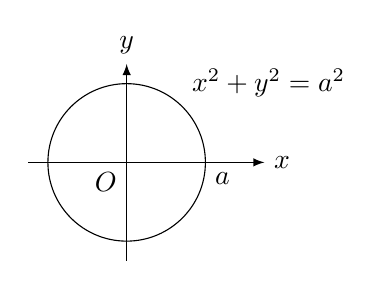
\begin{tikzpicture}
\draw[-latex](-1.25,0)--(1.75,0)node[right]{$x$};
\draw[-latex](0,-1.25)--(0,1.25)node[above]{$y$};
\draw (0,0) circle (1);
\draw(1,0)node[below right]{$a$};
\draw(0,0)node[below left]{$O$};
\draw(45:1)node[above right]{$x^2+y^2=a^2$};
\end{tikzpicture}
\caption{مساوات کی ترسیم}
\end{subfigure}%
\begin{subfigure}{0.5\textwidth}
\centering
\begin{tikzpicture}
\draw[fill=lgray] (0,0) circle (1);
\draw[-latex](-1.25,0)--(1.75,0)node[right]{$x$};
\draw[-latex](0,-1.25)--(0,1.25)node[above]{$y$};
\draw(1,0)node[below right]{$a$};
\draw(0,0)node[below left]{$O$};
\draw(45:1)node[above right]{$x^2+y^2\le a^2$};
\end{tikzpicture}
\caption{عدم مساوات کی ترسیم}
\end{subfigure}%
\caption{مساوات اور عدم مساوات کی ترسیم (مثال \حوالہ{مثال_ابتدائی_مساوات_عدم_مساوات_ترسیم})}
\label{شکل_مثال_ابتدائی_مساوات_عدم_مساوات_ترسیم}
\end{figure}
\انتہا{مثال}
%========================

اکائی رداس کا دائرہ جس کا مرکز مبدا ہو کو \اصطلاح{اکائی دائرہ}\فرہنگ{اکائی دائرہ}\حاشیہب{unit circle}\فرہنگ{unit circle} کہتے ہیں۔

\ابتدا{مثال}\شناخت{مثال_ابتدائی_قطع_مکافی}
مساوات \عددی{y=x^2} پر غور کریں۔\عددی{(0,0)}، \عددی{(1,1)}، \عددی{(-1,1)}، \عددی{(2,4)} اور \عددی{(-2,4)} ایسی چند نقطے ہیں جن کے محدد اس مساوات کو مطمئن کرتے ہیں۔یہ نقطے (اور ایسے تمام باقی نقطے جو اس مساوات کو مطمئن کرتے ہوں) مل کر ہموار منحنی دیتے ہیں جس کو \اصطلاح{قطع مکافی}\فرہنگ{قطع مکافی}\حاشیہب{parabola}\فرہنگ{parabola} کہتے ہیں (شکل \حوالہ{شکل_مثال_ابتدائی_قطع_مکافی})۔
\begin{figure}
\centering
\begin{tikzpicture}
\begin{axis}[small,axis lines*=middle,xlabel={$x$},ylabel={$y$},xlabel style={at={(current axis.right of origin)},anchor=north west}, ylabel style={rotate=-90},ylabel style={at={(current axis.above origin)},anchor=north east},ytick={1,4},yticklabels={$2$,$4$},xmax=2.9]
\addplot[domain=-2.2:2.2]{x^2}node[pos=0.75,right]{$y=x^2$};
\addplot[mark=none] plot coordinates {(0,0)}node[circ]{};
\addplot[mark=none] plot coordinates {(-2,4)}node[circ]{}node[right]{$(-2,4)$};
\addplot[mark=none] plot coordinates {(2,4)}node[circ]{}node[left]{$(2,4)$};
\addplot[mark=none] plot coordinates {(1,1)}node[circ]{}node[right]{$(1,1)$};
\addplot[mark=none] plot coordinates {(-1,1)}node[circ]{}node[left]{$(-1,1)$};
\end{axis}
\end{tikzpicture}
\caption{قطع مکافی (مثال \حوالہ{مثال_ابتدائی_قطع_مکافی})}
\label{شکل_مثال_ابتدائی_قطع_مکافی}
\end{figure}

\انتہا{مثال}
%============================
\جزوحصہء{سیدھے خطوط}
مستوی میں دو نقطوں \عددی{N_1(x_1,y_1)} اور \عددی{N_2(x_2,y_2)} سے یکتا سیدھا خط گزرتا ہے جس کو عموماً خط \عددی{N_1N_2} کہتے ہیں۔ 

مستوی میں کسی بھی غیر انتصابی خط پر ہر دو نقطوں \عددی{N_1(x_1,y_1)} اور \عددی{N_2(x_2,y_2)} کے لئے درج ذیل نسبت
\begin{align*}
m=\frac{\Delta y}{\Delta x}=\frac{y_2-y_1}{x_2-x_1}
\end{align*}
کی قیمت ایک جیسی ہو گی (شکل \حوالہ{شکل_ابتدائی_سیدھا_خط_ڈھلوان})۔
\begin{figure}
\centering
\begin{tikzpicture}
\pgfmathsetmacro{\ang}{30}
\pgfmathsetmacro{\xA}{0.5*cos(\ang)}
\pgfmathsetmacro{\xB}{1.5*cos(\ang)}
\pgfmathsetmacro{\xC}{3*cos(\ang)}
\pgfmathsetmacro{\xD}{4*cos(\ang)}
\pgfmathsetmacro{\yA}{0.5*sin(\ang)}
\pgfmathsetmacro{\yB}{1.5*sin(\ang)}
\pgfmathsetmacro{\yC}{3*sin(\ang)}
\pgfmathsetmacro{\yD}{4*sin(\ang)}
\draw[-latex](-0.5,0)--+(5,0)node[right]{$x$};
\draw[-latex](0,-0.25)--(0,2.5)node[above]{$y$};
\draw(-0.5,0.5)--++(\ang:5)node[above]{$L$};
\draw(-0.5,0.5)++(\ang:0.5)coordinate(kA)node[circ]{}++(\ang:1)coordinate(kB)node[circ]{}++(\ang:1.5)coordinate(kC)node[circ]{}++(\ang:1)coordinate(kD)node[circ]{};
\draw(kA)node[shift={(90+\ang:0.4)}]{$N_1'$};
\draw(kB)node[shift={(90+\ang:0.5)}]{$N_1(x_1,y_1)$};
\draw(kC)node[shift={(90+\ang:0.5)}]{$N_2(x_2,y_2)$};
\draw(kD)node[shift={(90+\ang:0.4)}]{$N_2'$};
\draw(kB)--++(\xC-\xB,0)node[pos=0.5,below]{$\Delta x$}coordinate(kE)node[shift={(0.15,-0.15)}]{$Q$};
\draw(kE)--++(0,\yC-\yB)node[pos=0.5,right]{$\Delta y$};
\draw(kA)--++(\xD-\xA,0)node[pos=0.5,below]{$\Delta x'$}coordinate(kF)node[shift={(0.15,-0.15)}]{$Q'$};
\draw(kF)--++(0,\yD-\yA)node[pos=0.5,right]{$\Delta y'$};
\end{tikzpicture}
\caption{$N_1QN_2$ اور $N_1'Q'N_2'$ متشابہ مثلثات ہیں لہٰذا $\tfrac{\Delta y}{\Delta x}=\tfrac{\Delta y'}{\Delta x'}$ ہو گا}
\label{شکل_ابتدائی_سیدھا_خط_ڈھلوان}
\end{figure}

\ابتدا{تعریف}
درج ذیل شرح
\begin{align*}
m=\frac{\Delta y}{\Delta x}=\frac{y_2-y_1}{x_2-x_1}
\end{align*}
غیر انتصابی خط \عددی{N_1N_2} کی \اصطلاح{ڈھلوان}\فرہنگ{ڈھلوان}\حاشیہب{slope}\فرہنگ{slope} کہلاتی ہے۔
\انتہا{تعریف}
%========================

ڈھلوان ہمیں خط کی چڑھائی یا اترائی دیتی ہے۔مثبت ڈھلوان کے خط پر دائیں رخ چلتے ہوئے چڑھائی نظر آئے گی جبکہ منفی ڈھلوان کے خط پر دائیں رخ چلتے ہوئے اترائی نظر آئے گی۔ڈھلوان کی مطلق قیمت جتنی زیادہ ہو چڑھائی یا اترائی اتنی زیادہ ہو گی۔انتصابی خط کی ڈھلوان کے لئے \عددی{\Delta x=0} ہو گا لہٰذا شرح \عددی{\tfrac{\Delta y}{\Delta x}} غیر معین ہو گا\حاشیہد{چونکہ \عددی{0} سے کسی بھی عدد کو تقسیم کرنا ممکن نہیں ہے۔}۔یوں انتصابی خط کی ڈھلوان غیر معین ہے۔ افقی خط کی ڈھلوان \عددی{0} ہے۔
